\section{Realisering og test}
\label{sec:research}

Punktprøvingsfrekvensen $f_s$ er satt til 6,4 kHz. Dermed blir spesifikasjonene som plottet i tabell \ref{tab:spec}. 

\begin{table}[ht]
    \caption{Filterspesifikasjoner}
    \centering
    \begin{tabular}{lll}
        \hline
        Spesifikasjon & Formel                              & Verdi        \\ \hline
        $f_s$         &                                     & 6400Hz       \\ 
        B             & $\frac{f_s}{2}$                     & 3200Hz       \\ 
        $f_c$         & $\geq\frac{3}{8}f_s$                & $\geq$2400Hz \\ 
    \end{tabular}
    \label{tab:spec}
\end{table}

Ved å ta i bruk formlene gitt i seksjon \ref{sec:concept} blir beregninene som vist i tabell \ref{tab:calculations}.

\begin{table}[hbt]
    \caption{Beregninger.}
    \centering
    % \setlength\extrarowheight{9pt}
    \begin{tabular}{lllll}
        \hline
        Størrelse   & Formel                                              & Måltall og enhet          & Realiserte verdier  & Avvik\\ \hline
        A           & $10^{\frac{A[dB]}{20}}$                             & $\approx0.3162$           &                     & \\ 
        n           & $\frac{1}{2}\frac{ln(A^{-2}-1)}{ln(\frac{f}{f_c})}$ & $\approx3.81\rightarrow4$ &                     & \\ 
        R           &                                                     & $1k\Omega$                & $1k\Omega$          & \\ 
        $\zeta_1$   & $\cos [\frac{\pi}{2n}+(i-1)\frac{\pi}{n}]$          & 0.92388                   &                     & \\ 
        $\zeta_2$   & $\cos [\frac{\pi}{2n}+(i-1)\frac{\pi}{n}]$          & 0.38268                   &                     & \\ 
        $\omega_0$  & $2\pi f_c$                                          & $15079.64\frac{rad}{s}$   &                     & \\ 
        $\tau_{11}$ & $\frac{1}{\omega_0 \zeta_1}$                        & $71.77\mu $s              &                     & \\ 
        $\tau_{12}$ & $\frac{1}{\omega_0^2 \tau_{11}}$                    & $61.27\mu $s              &                     & \\ 
        $\tau_{21}$ & $\frac{1}{\omega_0 \zeta_2}$                        & $173.29\mu $s             &                     & \\ 
        $\tau_{22}$ & $\frac{1}{\omega_0^2 \tau_{21}}$                    & $25.38\mu $s              &                     & \\ 
        $C_{11}$    & $\frac{\tau_{11}}{R}$                               & $71.77$nF                 &$71.32$nF            & 0.62\%\\ 
        $C_{12}$    & $\frac{\tau_{12}}{R}$                               & $61.27$nF                 &$61.65$nF            & 0.62\%\\ 
        $C_{21}$    & $\frac{\tau_{21}}{R}$                               & $173.29$nF                &$173.12$nF           & 0.10\%\\ 
        $C_{22}$    & $\frac{\tau_{22}}{R}$                               & $25.38$nF                 &$25.83$nF            & 1.74\%\\ 
        \end{tabular}
        \label{tab:calculations}
    \end{table}

Den realiserte kretsen er illustrert i figur \ref{fig:01realised} og fysisk oppkoblet i figur \ref{fig:03}. 

\begin{figure}[!h]
	\centering
	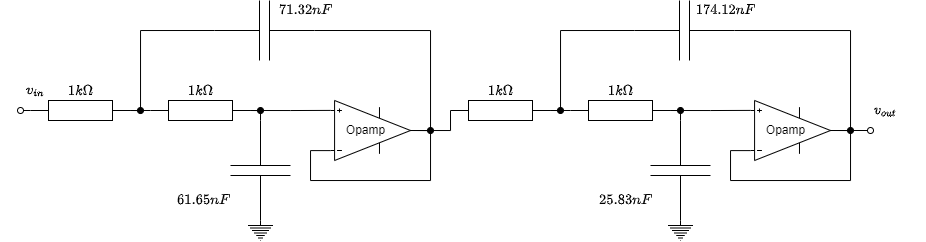
\includegraphics[scale=0.45]{./Images/03Research/01realisertkrets.png}
	\caption{Realisert krets med verdier.\cite{pham_2022_selvlaget}}
	\label{fig:01realised}
\end{figure}

Med denne kretsen ble frekvensresponsen lik figur \ref{fig:02frekvensresponsrealisert}.

\begin{figure}[!h]
	\centering
	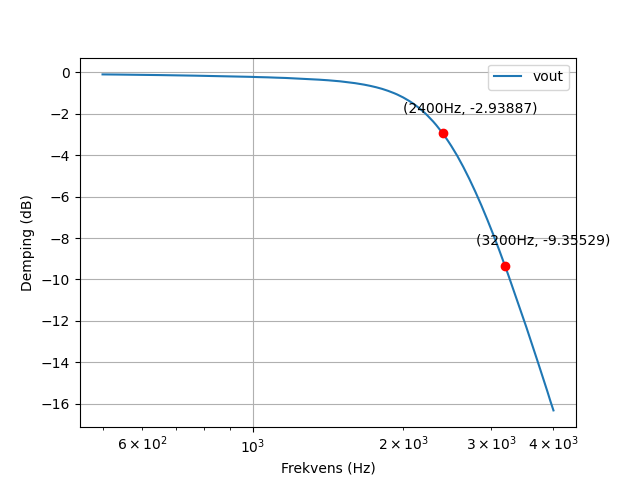
\includegraphics[scale=0.45]{./Images/03Research/02frekvensrespons.png}
	\caption{Frekvensrespons for realisert Anti-alias-filter.}
	\label{fig:02frekvensresponsrealisert}
\end{figure}

Det observeres at med disse komponentene så blir kravet om at knekkfrekvensen skal være $f_c\geq2400Hz$ oppfyllt, men ikke kravet om at dempingen ved $B=3200Hz$ er lavere enn 10dB. Ved å legge til 2,13 nF slik at $C_{22} = 27.96$ blir frekvensresponsen lik figur \ref{fig:02frekvensresponsrealisert2}. Dette er kan forklares med at ved å øke $C_{22}$, så får man en høyere $\tau_{22}$ som igjen fører til en lavere dempningsfaktor $\zeta_2$ ifølge formlene oppgitt i seksjon \ref{sec:Systemfunksjonen}. Ved bruk av formel \ref{eq:Q-faktor}  får man at $Q$ blir lavere der man kan se på figur \ref{fig:Qfaktor} at en får en mer dempet frekvensrespons på bekostning av båndbredden.

\begin{figure}[!h]
	\centering
	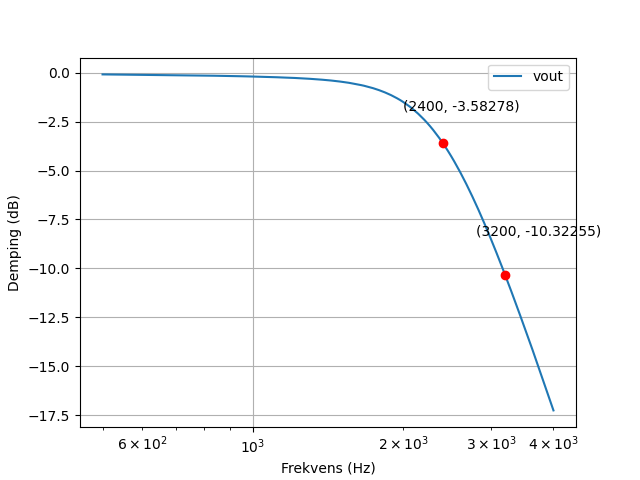
\includegraphics[scale=0.45]{./Images/03Research/02frekvensrespons2.png}
	\caption{Frekvensrespons for realisert Anti-alias-filter med  $C_{22}=27.96$.}
	\label{fig:02frekvensresponsrealisert2}
\end{figure}

Grunnen til at kravet om en doemping på minst 10 dB ved frekvensen $\frac{f_s}{2}$, og en knekkfrekvens på $f_c\geq 0.75\frac{f_s}{2}$ ikke blir realisert kan skyldes avvik i komponentene.

Det kan vurderes å øke ordenen på systemet i et forsøk om å få oppfylt kravene, som beskrevet i seksjon \ref{sec:Nødvendig_orden} og vist i figur \ref{fig:05order} ser man at mengden filteret får en økt dempning ved en høyere orden avtar med flere orden. Men siden det mangler kun -0.64471 dB for å oppnå kravet for B, så antas det at det ville holdt med en orden til da man ved bruk av formlene \ref{eq:magnitude} og \ref{eq:decibeltonone} får ville gått en dempning på -12.73 dB ved en 5. ordens Butterworth lavpassfilter. 

\begin{figure}[!h]
	\centering
	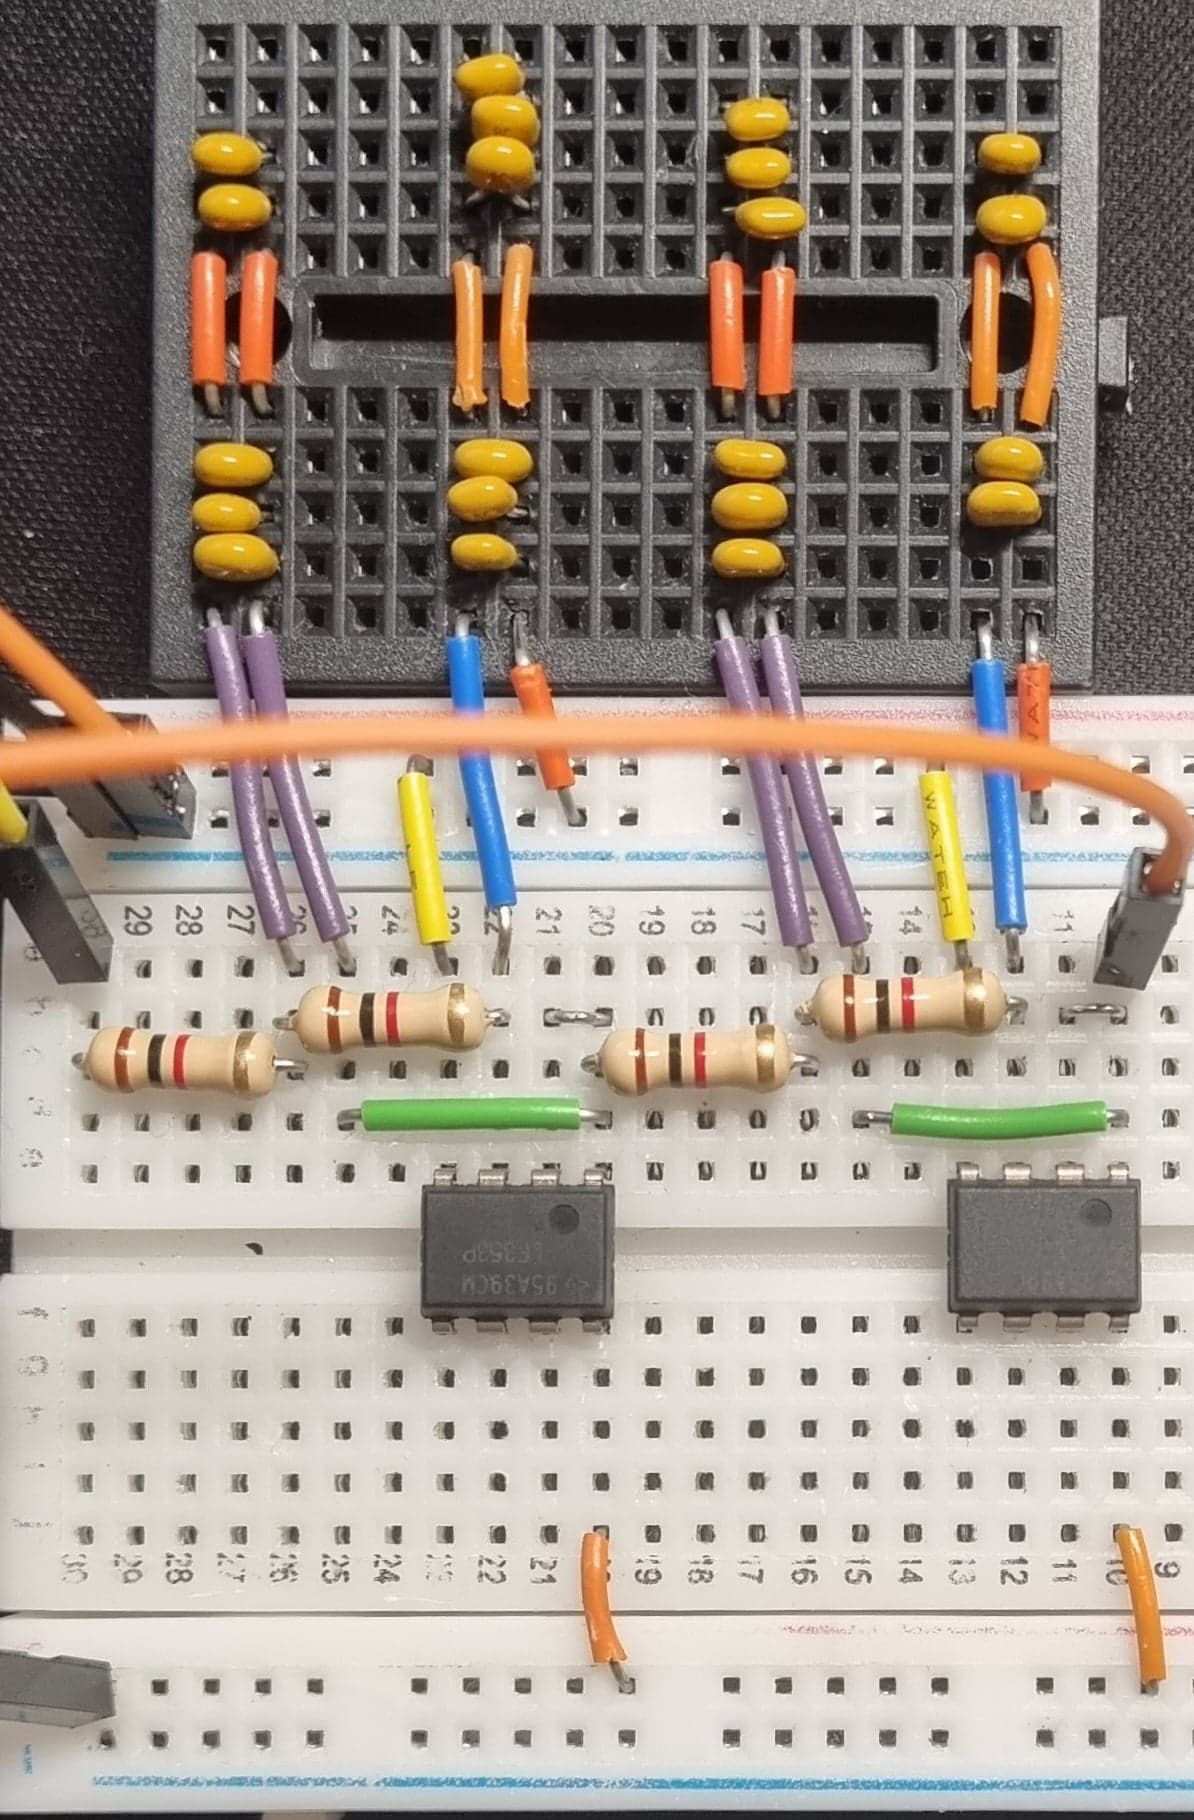
\includegraphics[scale=0.1]{./Images/03Research/03}
	\caption{Fysisk realisert krets.}
	\label{fig:03}
\end{figure}

\begin{equation}
    \Sigma
\end{equation}